
\chapter{Acoustique}

\section{Courbe de Wegel}
\label{acoustique}

<<Effectivement la courbe de Wegel est la courbe de réponse obtenue
lorsque sont posées en abscisses les fréquences, et en ordonnées ascendantes
les intensités. Un premier seuil s'obtient, en partie basse, suivant
un minimum qui commence dans les fréquences graves à environ 
\SIrange{40}{50}{\dB}, avoisine ensuite la courbe des abscisses entre 2000 et \SI{3000}{\Hz}
et redevient ascendante à \SI{40}{\decibel} / \SI{50}{\decibel} dans les aigus entre \SI{8000}{\Hz} et
\SI{10000}{\Hz}. Cette courbe se complète et prend l'allure de citron selon
l'expression qu'on lui confère lorsqu'on envoie des
sons d'intensité croissante et qu'on obtient alors une courbe des
seuils maxima qui se déterminent là où l'oreille commence à souffrir,
d'où le nom de ``seuil de la douleur". Ces seuils
commencent dans les graves, également de \SIrange{50}{60}{\decibel}, rejoignant la première
courbe, puis ils atteignent \SIrange{120}{130}{\decibel} entre \SI{2000}{\Hz} et \SI{3000}{\Hz} pour
chuter ensuite dans les aigus en rejoignant également la première
courbe. La ligne médiane qui se situe aux environs de \SIrange{50}{60}{\dB}, qui
est linéaire représente une zone dite ``Zone de Munsen''.
Elle répond à la dynamique de l'oreille, c'est-à-dire
à sa zone ``optimale" de fonctionnement sans
distorsion. Dans toutes les autres zones, l'oreille
agit comme un filtre dont les pentes sont variables en fonction de
l'intensité, avec un lieu de rotation situé de \SIrange{1000}{2000}{\Hz}. Pour pallier ces distorsions toujours difficiles à intégrer
dans la lecture des schémas, les Américains ont standardisé les audiogrammes
du type de ceux que nous utilisons tous en inversant l'image
de Wegel et en redressant les \emph{minima} pour obtenir une ligne droite.
Ces normes gardent néanmoins une zone préférentielle de \SIrange{1000}{2000}{\Hz} malgré les compensations de \SIrange{30}{40}{\dB} accordées sur la courbe,
dans les graves et les aigus.>>\autocite[Bernard Auriol, conversation, conférence]{auriol:conversation_conference}.

% OGA: stp la source bibliographique ou conférence

\section{Impédance}
\label{impedance}

Définition de l'impédance : L'impédance acoustique
caractérise la résistance qu'un milieu oppose à sa mise en mouvement
lorsqu'il est traversé par une onde acoustique. Elle est définie comme
le rapport de la pression acoustique sur la vitesse de déplacement
locale dans un milieu, et est généralement notée $Z$. Elle dépend de
la température. L'impédance caractéristique d'un milieu (solide, liquide
ou gazeux) est définie comme le rapport de la pression acoustique
sur la vitesse de déplacement en milieu ouvert (c'est-à-dire
en l'absence d'ondes réfléchies). L'impédance caractéristique est
une propriété du matériau considéré égale, dans le cas d'un espace
illimité, au produit de la masse volumique du matériau $\rho$
par la vitesse du son $c$ dans ce même matériau : $Z = \rho_{m} c$.

Unités : $\rho_{m}$ étant exprimé en \si{kg/m\cubed},
$c$ en \si{m/s}, $Z$ est
exprimé en \si{\pascal . s/m}.

\chapter{Privatklinik von Meiringen}



Information für Mitwirkende an der klinischen Studie
« Evaluierung des aktiven Hörvermögens »


Sehr geehrte Damen und Herren,

Herzlichen Dank für Ihr Interesse an dieser Studie !

Wozu dient diese Studie und weshalb werden Sie um eine Teilnahme gebeten ?

Während Ihrem Klinikaufenthalt  in der Privatklinik von Meiringen werden Sie im Kontext 
unseres multidisziplinären Teams verschiedene Therapien besuchen, unter anderem auch die Musiktherapie. Bei der vorliegenden Studie möchten wir untersuchen, wie sich die Musiktherapie auf Ihr Zuhörvermögen auswirkt.
Musiktherapie ist eine gut erforschte Intervention im Bereich des Depressions und Burnouts, da Sie ein relativ neues Berufsfeld ist, gibt es noch viel Forschungspotential.
Das Hörtest konnte sich als ein Instrument erweisen, um die Veränderung des Gehörs des Patienten bei einer Musiktherapiebehandlung zu beweisen. Die Verbindung dieses Ansatzes mit der Musiktherapie ist noch nicht erforscht und daher soll dieser Ansatz wissenschaftlich näher untersucht werden.
Wenn Sie keine Musiktherapie besuchen aber Interesse für diese Studie haben, sind Sie herzlich eingeladen, dieses Test zu tun. Im Rahmen under MAS brauchen wir unbedingt eine Kontrollgruppe.

Wie sieht eine Teilnahme an der Studie aus ?

Die Untersuchung erfolgt sehr einfach in mehreren Schritten.
Zu Verfügung steht ein Apparat, mit dem sich spezifische Hörtests durchführen lassen.
Allgemein Verlauf des Tests :  
Sie hören einen sehr leisen Ton mit Zuhörern zu und werden ihn entweder mit der rechten  oder linken Hand  signalisieren. Das dauert ungefähr 30 Minuten.
Es wird zwei Tests geben : ein vor der Therapie und ein nach der Therapie.
Wir bitten Sie auch, eine kleine Fragebogen zu erfüllen.


Falls Sie Fragen haben, dürfen Sie sich gerne via E-Mail melden : valerie.gaillard\@gmx.ch

Wir bedanken uns herzlich für Ihre Zeit und die Teilnahme an dieser Studie.


Valérie Gaillard

 Le matériel utilisé : une table, deux chaises, l'appareil
test Hearing et les écouteurs aériens et osseux, un crayon, deux
feutres ( rouge et bleu), une feuille avec la grille de fréquences à
remplir.

ZhdK : Upgrade MAS Klinische Musiktherapie 15-17

\chapter{Questionnaires}

\includepdfmerge{French_WHOQOL-BREF.pdf, -, 
	WHOQOLALLEMANDBREFupdated.pdf, -}


%\section{Questionnaire 1}
%
%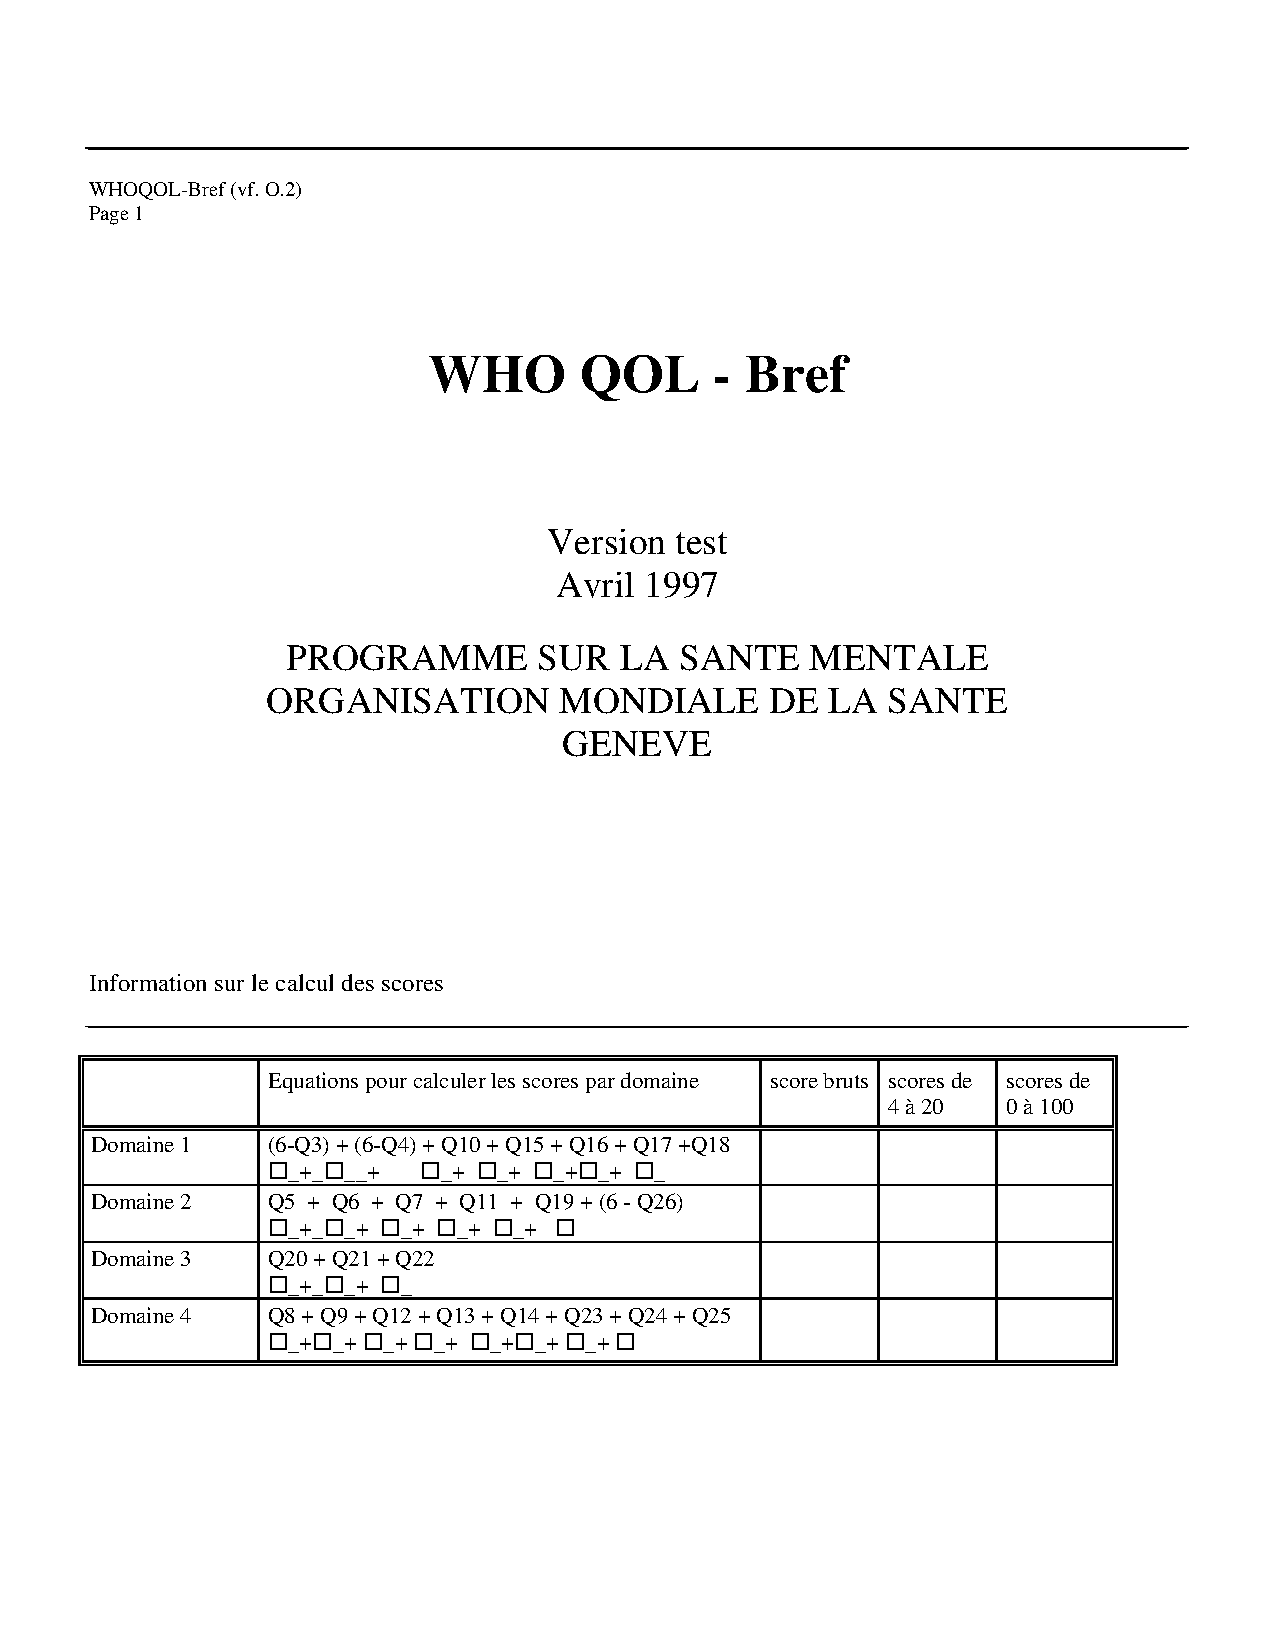
\includepdf[pages=-]{French_WHOQOL-BREF.pdf}
%
%\section{Questionnaire 2}
%
%
\includepdf[pages=-]{WHOQOLALLEMANDBREFupdated.pdf}
